\section{Concepto de Observatorio Virtual}

\emph{``En la actualidad se está generando una ingente cantidad de datos
provenientes de un número creciente de instrumentos astronómicos con cada vez
mejor resolución, lo que está multiplicando las neceisdades de almacenamiento''.}
\footnote{El Observatorio virtual, Por Juan de Dios Santander (IAA-CSIC)}

Esta frase refleja problemáticas que se presentan a la actualidad, pero desde
otro punto de vista también son oportunidades de cubrir ciertas necesidades.
Algunas necesidades son:
%\emph{Algunas de estas son}:

%\todo{Resaltar la palabra o palabras antes del ``:'', con negrita o emph}
\begin{itemize}
	\item Facilidad de acceso: en el mundo existen distintos instrumentos
		astronómicos, los cuales generan volúmenes de datos a gran escala,
		por lo que es necesario unificar la forma en que se publica esta información
		de tal modo que no sea difícil encontrar los detalles requeridos.
	\item Información relativa a los datos: cuando se habla de datos en
		astronomía es necesario entender el contexto en el cual se desenvuelven.
		Los datos en astronomía pueden ser listas de números, matrices de números
		(píxeles de una imagen por ejemplo) o arreglos de más de dos dimensiones.
		Si una persona, independiente que sea astrónomo, busca cierto
		conjunto de datos, necesita saber cómo hacerlo, es decir,
		qué parámetros, campos, descripciones poseen los mismos.
		Respecto a esto, en astronomía se han generado distintos formatos
		de datos astronómicos, por ejemplo, ``Flexible Image Transport System''\cite{fits_definition}
		(FITS).	La necesidad en cuestión es que los datos elaborados por un grupo de
		investigación pueda ser utilizado por cualquier otro.
	\item Procesamiento de datos: algunos datos, al poseer volúmenes grandes,
		necesitan ciertas capacidades de almacenamiento \cite{archive_tsunami} y cómputo \cite{data_hpc}.
		Por lo que los VO's ayudan a reducir la transferencia de información.
	\item Minería de datos: los datos son una fuente de valor importante para los
		astrónomos y científicos en general, por lo que constantemente se hacen esfuerzos
		en enriquecerlos. La manera en que se hace este proceso, es usando técnicas de 
		minería de datos \cite{vo_data_mining}, \emph{para}: reconocimiento de patrones, priorización
		de información, clasificación de estrellas, representatividad de datos, etc.;
		Por lo que es necesario proveer algoritmos que cumplan dicha labor.
		%\todo{Me esperaba mas información
		%    acá, debido aque el data mining o creacion de algoritmos que hagan tareas
		%    automáticas es y sera nuestro fuerte}
	\item Notificación y registro de servicios y datos nuevos: los datos
		disponibles estén permanentemente actualizados.
\end{itemize}

%Las necesidades que surgieron desde la comunidad astronómica y el
%aprovechamiento de las oportunidades que emergirían de las mismas, incentivó
%a la creación de una alianza internacional: la IVOA.
Al ir apareciendo distintas necesidades en la comunidad astronómica, se creó una alianza internacional entre 
distintos centros de investigación para aprovechar las oportunidades que fueron
apareciendo. Con esto nació IVOA.

\subsection{Protocolos y estándares IVOA}

IVOA fue formada en Junio del 2002.  \emph{Su misión es facilitar la
coordinación y colaboración necesaria para facilitar el acceso global e
integrado a los datos recogidos por los observatorios astronómicos
internacionales}.

Su principal función en la actualidad es crear, versionar y mantener informada
a la comunidad acerca de los protocolos y estándares \cite{ivoa_documents} a
usar.  Eso lo llevan a cabo mediante los Working Groups. Ellos preparan
documentos disponibles para toda la comunidad, los cuales describen distintas
funcionalidades, arquitecturas, normas, etc. para un observatorio virtual.
El diagrama de cómo se crean estos estándares está representado
en la figura~\ref{fig:creacionestandares}.
\begin{figure}[h!t]
        \centering
         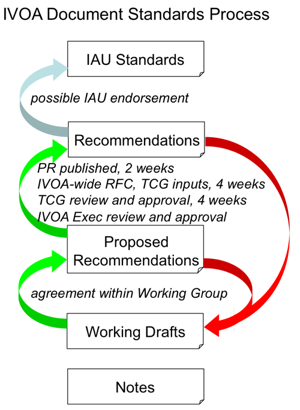
\includegraphics[width=0.45\textwidth]{img/diagrama_proceso.png}
         \caption{Creación de Estándares IVOA}
        \label{fig:creacionestandares}
\end{figure}

%\todo{poner esto como itemize, enumerate, o description, así se ve super feo}
Los \textbf{Working Groups} se encargan de elaborar
o versionar los estándares que se subdividen en \emph{áreas técnicas}\cite{reuna}: \\
\begin{itemize}
	\item
\textbf{Aplicaciones}\footnote{http://wiki.ivoa.net/twiki/bin/view/IVOA/IvoaApplications}:
se encarga de las herramientas de software que los astrónomos utilizan en su
labor para acceder a los datos y servicios. \\
	\item \textbf{Capa de acceso a los
datos}\footnote{http://wiki.ivoa.net/twiki/bin/view/IVOA/IvoaDAL}: definen y
formulan estándares para el acceso remoto a los datos. Se orientan a funciones
para clientes y publishers. \\
	\item \textbf{Modelamiento de
datos}\footnote{http://www.ivoa.net/twiki/bin/view/IVOA/IvoaDataModel}:
proporcionan un marco para la descripción de los metadatos asociados a los
datos observados (o simulados). Se orientan a relaciones lógicas entre esos
metadatos y el modo en que los astrónomos quieren examinar. \\
	\item \textbf{Grid y servicios
web}\footnote{http://wiki.ivoa.net/twiki/bin/view/IVOA/IvoaGridAndWebServices}:
definen el uso de tecnología de redes y servicios de Internet dentro del
contexto de VO. \\
	\item \textbf{Registro de
recursos}\footnote{http://wiki.ivoa.net/twiki/bin/view/IVOA/IvoaResReg}: define
la estructura y la interfaz de un \textit{IVOA Registry}. Permite a los
astrónomos localizar y hacer uso de recursos de VO. \\
	\item
\textbf{Semánticas}\footnote{http://wiki.ivoa.net/twiki/bin/view/IVOA/IvoaSemantics}:
exploran el significado o las interpretaciones de palabras o frases, o de otro
tipo de lenguaje en el contexto de astronomía, como por ejemplo, ontologías. \\
	\item \textbf{Eventos
VO}\footnote{http://wiki.ivoa.net/twiki/bin/view/IVOA/IvoaVOEvent}: define el
contenido y el significado de un paquete de información acerca de un evento
celestial transitorio como el paso de un cometa, entre otros. \\
\end{itemize}
